\documentclass[a4paper,12pt]{report}

\usepackage{cmap}
\usepackage[T2A]{fontenc}
\usepackage[utf8]{inputenc}
\usepackage[english,russian]{babel}
\usepackage{listings}
\usepackage{amsmath}
\usepackage{float}
\usepackage{csquotes}
\usepackage{mathtools}
\usepackage{hyphenat}
\usepackage{amsfonts}

\usepackage{xcolor}
\usepackage{hyperref}

\usepackage{graphicx}
\graphicspath{ {./images/} }

\definecolor{dkgreen}{rgb}{0,0.6,0}
\definecolor{gray}{rgb}{0.5,0.5,0.5}
\definecolor{mauve}{rgb}{0.58,0,0.82}

\lstset{
    language=Python,                
    basicstyle=\small\sffamily,
    numbers=left,               
    numberstyle=\tiny,         
    stepnumber=1,                   
    numbersep=5pt,                
    aboveskip=3mm,
    belowskip=3mm,
    showstringspaces=false,
    columns=flexible,
    captionpos=b, 
    basicstyle={\small\ttfamily},
    numbers=left,
    numberstyle=\tiny\color{gray},
    keywordstyle=\color{blue},
    commentstyle=\color{mauve},
    stringstyle=\color{dkgreen},
    breaklines=true,
    breakatwhitespace=true,
    tabsize=3
}

\title{Лабораторная работа №4\\Шум}
\author{Смирнов Никита}
\date{\today}

\begin{document}

\maketitle
\tableofcontents
\listoffigures
\lstlistoflistings

\maketitle

\chapter{Теоретическая часть}
\section{Общие сведения}

Преобразование Фурье функции $f$ вещественной переменной является интегральным и задаётся следующими формулами: 
    
\[
    \begin{aligned}
        \text{Прямое: } && F(\nu) &= \int_{-\infty}^{\infty} f(t) e^{-2\pi i\nu t} dt \\
        \text{Обратное: } && f(t) &=  \int_{-\infty}^{\infty} F(\nu) e^{2\pi i\nu t} d\nu
    \end{aligned}
\]

\section{Свойства}
\subsection{Линейность}
    
По определению, для некоторого векторного пространства $(V,K,+,\cdot)$, $a,b \in V$, $\gamma \in K$:

\[
    \begin{aligned}
        f: V \rightarrow V \text{ - линейна}
        \Longleftrightarrow
        \begin{cases}
                \gamma\cdot f(a) = f(\gamma\cdot a) \\
                f(a) + f(b) = f(a + b)
        \end{cases}
    \end{aligned}
\]
    
Очевидно, что преобразование Фурье (ПФ) удовлетворяет этому условию (как функция на $(\mathbb{R} \rightarrow \mathbb{R},\mathbb{C},+,\cdot)$), а следовательно:

\[
    \begin{aligned}
        Fourier\left(\sum_{i}\alpha_i\phi_i(t)\right)
        &= \sum_{i}\alpha_i \cdot Fourier(\phi_i(t)) \\
        &= \sum_{i}\alpha_i \Phi_i(\nu)
    \end{aligned}
\]

\subsection{Смещение функции}

При смещении функции $\phi(t)$ на $\Delta t$ результат ПФ умножается на $e^{2\pi i \nu\Delta t}$. Пусть $t' = t + \Delta t$, тогда:

\[
    \begin{aligned}
        Fourier\left(\phi(t + \Delta t)\right)
        &= \int_{-\infty}^{\infty} \phi(t + \Delta t) e^{-2\pi i\nu t} dt \\
        &= \int_{-\infty}^{\infty} \phi(t') e^{-2\pi i\nu (t' - \Delta t)} dt
    \end{aligned}
\]

Так как $dt' = d(t + \Delta t) = dt$, то:

\[
    \begin{aligned}
        \int_{-\infty}^{\infty} \phi(t') e^{-2\pi i\nu (t' - \Delta t)} dt'
        &= e^{2\pi i\nu\Delta t} \cdot \int_{-\infty}^{\infty} \phi(t') e^{-2\pi i\nu t'} dt' \\
        &= e^{2\pi i\nu\Delta t} \cdot F(\nu)
    \end{aligned}
\]

\subsection{Масштабирование функции}

Пусть $t' = \alpha t$, тогда:

\[
    \begin{aligned}
        Fourier\left(\phi(\alpha t)\right)
        &= \int_{-\infty}^{\infty} \phi(\alpha t) e^{-2\pi i\nu t} dt \\
        &= \int_{-\infty}^{\infty} \phi(t') e^{-2\pi i\nu \frac{t'}{\alpha}} dt
    \end{aligned}
\]

Так как $dt' = \alpha dt$, то для $a > 0$:

\[
    \begin{aligned}
        \int_{-\infty}^{\infty} \phi(t') e^{-2\pi i\nu \frac{t'}{\alpha}} dt
        &= \frac{1}{\alpha} \int_{-\infty}^{\infty} \phi(t') e^{-2\pi i\frac{\nu}{\alpha} t'} dt \\
        &= \frac{1}{\alpha} \Phi\left(\frac{\nu}{\alpha}\right)
    \end{aligned}
\]

Для $a < 0$ получится $dt' < 0$ при $dt > 0$. При этом нужно поменять пределы интегрирования местами, тогда получим результат с отрицательным знаком:

\[
    \begin{aligned}
        -\frac{1}{\alpha} \Phi\left(\frac{\nu}{\alpha}\right)
    \end{aligned}
\]

Таким образом, в одной форме это:

\[
    \begin{aligned}
        \frac{1}{\left|\alpha\right|} \Phi\left(\frac{\nu}{\alpha}\right)
    \end{aligned}
\]

Вывод: при сжатии функции по времени в $\alpha$ раз, её ПФ расширяется по частоте в $\alpha$ раз.

\subsection{Перемножение функции}

ПФ произведения двух функций - это свёртка их ПФ.

\[
    \begin{aligned}
        Fourier\left(\phi(t)\xi(t)\right) 
        &= \int_{-\infty}^{\infty} \phi(t)\xi(t) e^{-2\pi i\nu t} dt \\
        &= \int_{-\infty}^{\infty} \left( \int_{-\infty}^{\infty} \Phi(k) e^{2\pi i kt} dk \right) \xi(t) e^{-2\pi i\nu t} dt \\
        &= \int_{-\infty}^{\infty} \Phi(k) \left( \int_{-\infty}^{\infty} \xi(t) e^{2\pi i (k - \nu)t} dt \right) dk \\
        &= \int_{-\infty}^{\infty} \Phi(k) \left( \int_{-\infty}^{\infty} \xi(t) e^{-2\pi i (\nu - k)t} dt \right) dk \\
        &= \int_{-\infty}^{\infty} \Phi(k) \Xi(\nu - k) dk \\
        &= \left(\Phi * \Xi\right)(\nu)
    \end{aligned}
\]

\subsection{Свёртывание функции}
ПФ свёртки двух функций есть произведение ПФ этих функций. Доказывается аналогично в силу \textquote{симметрии} прямого и обратного преобразований Фурье.

\subsection{Дифференцирование функции}

При дифференцировании $\phi(t)$ по $t$ её ПФ умножается на $2\pi i \nu$.

\[
    \begin{aligned}
        Fourier\left(\frac{d\phi(t)}{dt}\right) 
        &= \int_{-\infty}^{\infty} \frac{d\phi(t)}{dt} e^{-2\pi i\nu t} dt \\
        &= \int_{-\infty}^{\infty} e^{-2\pi i\nu t} d\phi(t) \\
        &= \phi(t) e^{-2\pi\nu t} \bigg|_{-\infty}^{\infty} - \int_{-\infty}^{\infty} \phi(t) d\left(e^{-2\pi i\nu t}\right) \\
        &= \phi(t) e^{-2\pi\nu t} \bigg|_{-\infty}^{\infty} + 2\pi i\nu \int_{-\infty}^{\infty} \phi(t) e^{-2\pi i\nu t} dt \\
        &= \phi(t) e^{-2\pi\nu t} \bigg|_{-\infty}^{\infty} + 2\pi i\nu \cdot \Phi(\nu) \\
    \end{aligned}
\]

Прямое и обратное преобразование Фурье существует для функций с ограниченной энергией, то есть:

\[
    \begin{aligned}
        \int_{-\infty}^{\infty} |\phi(t)|^2 dt \neq \infty
    \end{aligned}
\]

И из этого следует, что первое слагаемое равно 0.

\subsection{Интегрирование функции}

При интегрировании ПФ делится на $2\pi i \nu$.

\[
    \begin{aligned}
        Fourier\left(\int_{-\infty}^{t} \phi(t') dt'\right) 
        &= \int_{-\infty}^{\infty} \left( \int_{-\infty}^{t} \phi(t') dt' \right) e^{-2\pi i\nu t} dt \\
        &= -\frac{1}{2\pi i\nu} \cdot \int_{-\infty}^{\infty} \left( \int_{-\infty}^{t} \phi(t') dt' \right) d\left(e^{-2\pi i\nu t}\right) \\
        &= -\frac{1}{2\pi i\nu} \cdot \left[ e^{-2\pi i\nu t} \int_{-\infty}^{t} \phi(t') dt' \biggr|_{-\infty}^{\infty} - \int_{-\infty}^{\infty} e^{-2\pi i\nu t} d\left(\int_{-\infty}^{t} \phi(t') dt'\right)\right] \\
        &= -\frac{1}{2\pi i\nu} \cdot \left[ e^{-2\pi i\nu t} \int_{-\infty}^{t} \phi(t) dt \biggr|_{-\infty}^{\infty} - \int_{-\infty}^{\infty} e^{-2\pi i\nu t} \phi(t) dt\right] \\
        &= -\frac{1}{2\pi i\nu} \cdot \left[ 0 - \int_{-\infty}^{\infty} e^{-2\pi i\nu t} \phi(t) dt\right] \\
        &= \frac{1}{2\pi i\nu} \cdot \int_{-\infty}^{\infty} e^{-2\pi i\nu t} \phi(t) dt \\
        &= \frac{1}{2\pi i\nu} \cdot \Phi(\nu)
    \end{aligned}
\]

0 возникает потому, что $\int_{-\infty}^{\infty} \phi(t') dt' = 0$.

\subsection{Обратимость}

Преобразования обратимы, причём обратное преобразование имеет практически такую же форму, как и прямое преобразование.

\chapter{Упражнение 4.1}
В этом упражениии необходимо скачать звук  источников шума. Определить похож ли спектр мощности скаченного звука на белый розовый или броуновский шумы.

Я нашел звук обстановки в ресторане.

\begin{lstlisting}[caption=Прослушивание скачанного шума]
import thinkdsp

wave = thinkdsp.read_wave('matias.wav')
wave.make_audio()
\end{lstlisting}

Выбрал отрезок:

\begin{lstlisting}[caption=Выбор короткого отрезка]
segment = wave.segment(start=5, duration=1.0)
segment.make_audio()
\end{lstlisting}

Посмотрим на спектр.

\begin{lstlisting}[caption=Спектр звука]
spectrum = segment.make_spectrum()
spectrum.plot_power()
decorate(xlabel='Frequency (Hz)')
\end{lstlisting}

\begin{figure}[H]
        \centering
        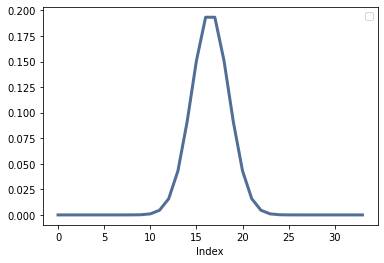
\includegraphics[width=0.75\textwidth]{1.png}
        \caption{Спектр звука}
        \label{fig:lab4_fig1_1}
\end{figure}

Амплитуда падает с частотой, поэтому это может быть красный или розовый шум. Мы можем проверить это, посмотрев на спектр мощности в логарифмической шкале.

\begin{lstlisting}[caption=Спектр мощности звука]
spectrum.plot_power()
decorate(xlabel='Frequency (Hz)',
                 xscale='log', 
                 yscale='log')
\end{lstlisting}

\begin{figure}[H]
        \centering
        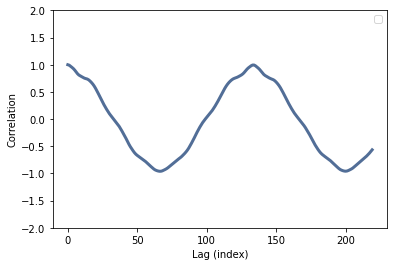
\includegraphics[width=0.75\textwidth]{2.png}
        \caption{Спектр мощности звука}
        \label{fig:lab4_fig1_2}
\end{figure}

Эта структура с увеличением, а затем и с уменьшением амплитуды кажется обычным явлением для естественных источников шума. Чтобы увидеть, как спектр меняется с течением времени, я выберу другой сегмент.

\begin{lstlisting}[caption=Выбор другого сегмента звука]
segment2 = wave.segment(start=2.5, duration=1.0)
segment2.make_audio()
\end{lstlisting}

Теперь рассмотрим два спектра:

\begin{lstlisting}[caption=Спектр двух звуков]
spectrum2 = segment2.make_spectrum()
spectrum.plot_power()
spectrum2.plot_power(color='#beaed4')
decorate(xlabel='Frequency (Hz)',
                 ylabel='Amplitude')
\end{lstlisting}

\begin{figure}[H]
        \centering
        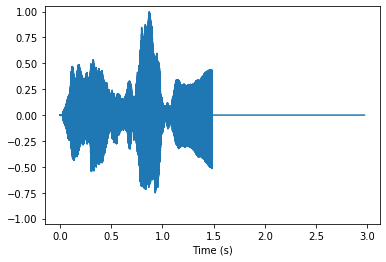
\includegraphics[width=0.75\textwidth]{3.png}
        \caption{Спектр двух звуков}
        \label{fig:lab4_fig1_3}
\end{figure}

Теперь рассмотрим график мощности в логарифмическом масштабе.

\begin{lstlisting}[caption=Спектр мощности двух звуков]
spectrum.plot_power()
spectrum2.plot_power(color='#beaed4')
decorate(xlabel='Frequency (Hz)',
                 ylabel='Amplitude',
                 xscale='log', 
                 yscale='log')
\end{lstlisting}

\begin{figure}[H]
        \centering
        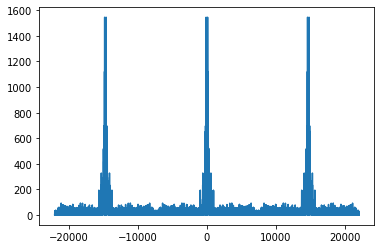
\includegraphics[width=0.75\textwidth]{4.png}
        \caption{Спектр мощности двух звуков}
        \label{fig:lab4_fig1_4}
\end{figure}

Таким образом, структура кажется неизменной с течением времени. Мы также можем посмотреть на спектрограмму:

\begin{lstlisting}[caption=Спектрограмма звука]
segment.make_spectrogram(512).plot(high=5000)
\end{lstlisting}

\begin{figure}[H]
        \centering
        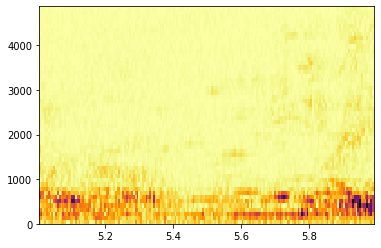
\includegraphics[width=0.75\textwidth]{5.png}
        \caption{Спектрограмма звука}
        \label{fig:lab4_fig1_5}
\end{figure}

В этом сегменте общая амплитуда падает, но смесь частот кажется стабильной.

\chapter{Упражнение 4.2}

\texttt{bartlett\_method} создает спектрограмму и извлекает \texttt{spec\_map}, который отображает время на объекты Spectrum. Он вычисляет PSD для каждого спектра, складывает их и помещает результаты в объект Spectrum.

\begin{lstlisting}[caption=Функция bartlett\_method]
def bartlett_method(wave, length=512, flag=True):
    spectro = wave.make_spectrogram(length, flag)
    spectrums = spectro.spec_map.values()
    psds = [spectrum.power for spectrum in spectrums]
    hs = np.sqrt(sum(psds) / len(psds))
    fs = next(iter(spectrums)).fs
    spectrum = thinkdsp.Spectrum(hs, fs, wave.framerate)
    return spectrum
\end{lstlisting}

Построим сегменты:

\begin{lstlisting}[caption=Сегменты звуков]
psd = bartlett_method(segment)
psd2 = bartlett_method(segment2)

psd.plot_power()
psd2.plot_power(color='#beaed4')

decorate(xlabel='Frequency (Hz)', 
                 ylabel='Power', 
                 xscale='log', 
                 yscale='log')
\end{lstlisting}

\begin{figure}[H]
        \centering
        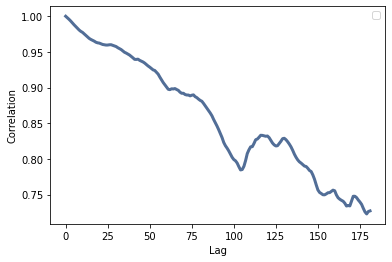
\includegraphics[width=0.75\textwidth]{6.png}
        \caption{Сегменты звуков}
        \label{fig:lab4_fig2_1}
\end{figure}

Теперь мы можем более чётко увидеть взаимосвязь между мощностью и частотой. Это не простая линейная зависимость, но она одинакова для разных сегментов, таких как около 1000 Гц, 6000 Гц и выше 10000 Гц.
\chapter{Упражнение 4.3}

На предложенной веб-странице я скачал данные о ежедневной цене \texttt{BitCoin} в течение года.

\begin{lstlisting}[caption=Таблица данных]
data = pd.read_csv('BTC_USD_2020-04-08_2021-04-07-CoinDesk.csv')
data
\end{lstlisting}

\begin{figure}[H]
        \centering
        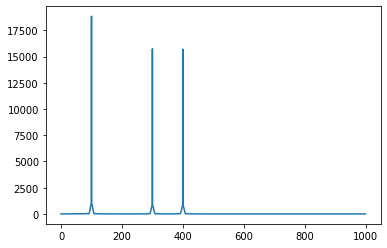
\includegraphics[width=0.75\textwidth]{7.png}
        \caption{Таблица данных}
        \label{fig:lab4_fig3_1}
\end{figure}

Визуализируем скачанные данные.

\begin{lstlisting}[caption=Визуализация данных]
wave = thinkdsp.Wave(data['Closing Price (USD)'], data.index, framerate=1)
wave.plot()
decorate(xlabel='Time (days)')
\end{lstlisting}

\begin{figure}[H]
        \centering
        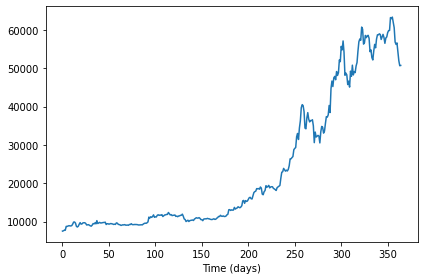
\includegraphics[width=0.75\textwidth]{8.png}
        \caption{Визуализация данных}
        \label{fig:lab4_fig3_2}
\end{figure}

Построим спектр искусственно созданного звука, где частотой будет выступать 1/дни.

\begin{lstlisting}[caption=Спектр искусственного звука]
spectrum = wave.make_spectrum()
spectrum.plot_power()
decorate(xlabel='Frequency (1/days)',
                 xscale='log', yscale='log')
\end{lstlisting}

\begin{figure}[H]
        \centering
        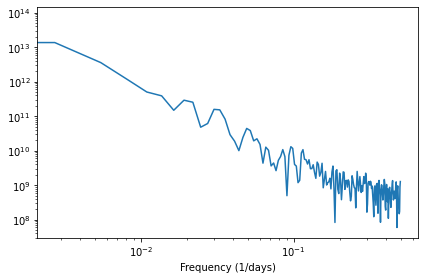
\includegraphics[width=0.75\textwidth]{9.png}
        \caption{Спектр искусственного звука}
        \label{fig:lab4_fig3_3}
\end{figure}

Спектр сход с прямой линией, поэтому можно предположить, что это "красный" или "розовый" шум. Проверим это, узнав наклон прямой.

\begin{lstlisting}[caption=Наклон прямой]
spectrum.estimate_slope()[0]
\end{lstlisting}

Наклон составляет \texttt{-1.8582636508741062}, что похоже на красный шум (который должен иметь наклон -2).

\chapter{Упражнение 4.4}

Созданный класс \texttt{UncorrelatedPoissonNoise} представляет некоррелированный пуассоновский шум. Оценивает сигнал в заданное время.

\begin{lstlisting}[caption=Созданный класс UncorrelatedPoissonNoise]
class UncorrelatedPoissonNoise(thinkdsp.Noise):
    def evaluate(self, ts):
        ys = np.random.poisson(self.amp, len(ts))
        return ys
\end{lstlisting}

Рассмотрим как это звучит при низких уровнях «радиации».

\begin{lstlisting}[caption=Создание звука]
amp = 0.001
framerate = 10000
duration = 1

signal = UncorrelatedPoissonNoise(amp=amp)
wave = signal.make_wave(duration=duration, framerate=framerate)
wave.make_audio()
\end{lstlisting}

Звук действительно похож на звуки от счётчика Гейгера, будто бы находишься где-то в Припяти. Чтобы убедиться, что все работает, мы сравниваем ожидаемое количество частиц и фактическое количество:

\begin{lstlisting}[caption=Создание звука]
expected = amp * framerate * duration
actual = sum(wave.ys)
print(expected, actual)
\end{lstlisting}

Количество частиц в обоих случаях равняется 10. Теперь рассмотрим полученный звук:

\begin{lstlisting}[caption=Визуализация звука]
wave.plot()
\end{lstlisting}

\begin{figure}[H]
        \centering
        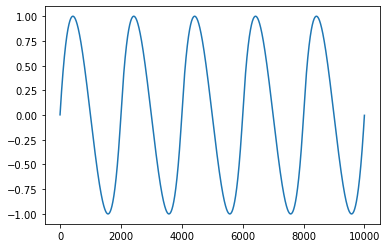
\includegraphics[width=0.75\textwidth]{10.png}
        \caption{Визуализация звука}
        \label{fig:lab4_fig4_1}
\end{figure}

Рассмотрим спектр мощности в логарифмическом масштабе:

\begin{lstlisting}[caption=Спектр мощности звука]
spectrum = wave.make_spectrum()
spectrum.plot_power()
decorate(xlabel='Frequency (Hz)',
                 ylabel='Power',
                 xscale='log', 
                 yscale='log')
\end{lstlisting}

\begin{figure}[H]
        \centering
        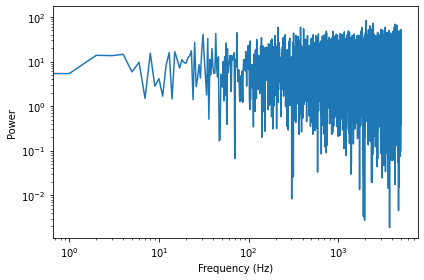
\includegraphics[width=0.75\textwidth]{11.png}
        \caption{Спектр мощности звука}
        \label{fig:lab4_fig4_2}
\end{figure}

Рассмотрим наклон:

\begin{lstlisting}[caption=Наклон прямой]
spectrum.estimate_slope().slope
\end{lstlisting}

Похоже на белый шум, а крутизна близка к 0 (\texttt{-0.004513262607615736}).

При более высокой скорости поступления это больше похоже на белый шум:

\begin{lstlisting}[caption=Создание нового звука]
amp = 1
framerate = 10000
duration = 1

signal = UncorrelatedPoissonNoise(amp=amp)
wave = signal.make_wave(duration=duration, framerate=framerate)
wave.make_audio()
\end{lstlisting}

Построим его график.

\begin{lstlisting}[caption=Визуализация нового звука]
wave.plot()
\end{lstlisting}

\begin{figure}[H]
        \centering
        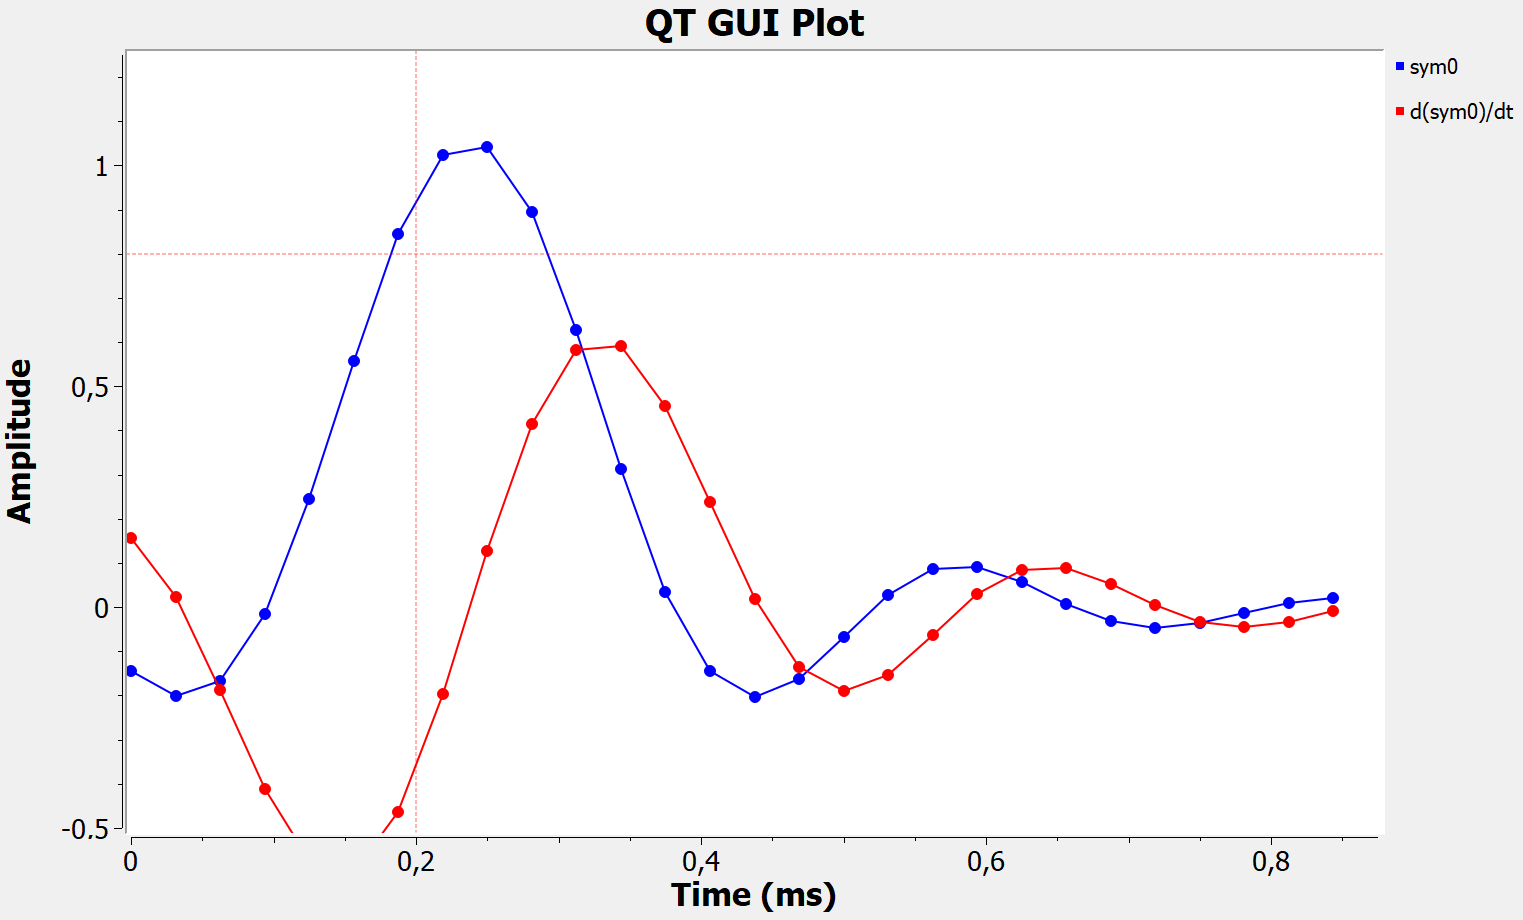
\includegraphics[width=0.75\textwidth]{12.png}
        \caption{Визуализация нового звука}
        \label{fig:lab4_fig4_3}
\end{figure}

И спектр сходится на гауссовском шуме.

\begin{lstlisting}[caption=Сравнение спектров]
spectrum = wave.make_spectrum()
spectrum.hs[0] = 0

thinkplot.preplot(2, cols=2)
thinkstats2.NormalProbabilityPlot(spectrum.real, label='real')
thinkplot.config(xlabel='Normal sample',
                 ylabel='Power',
                 legend=True,
                 loc='lower right')

thinkplot.subplot(2)
thinkstats2.NormalProbabilityPlot(spectrum.imag, label='imag')
thinkplot.config(xlabel='Normal sample',
                     loc='lower right')
\end{lstlisting}

\begin{figure}[H]
        \centering
        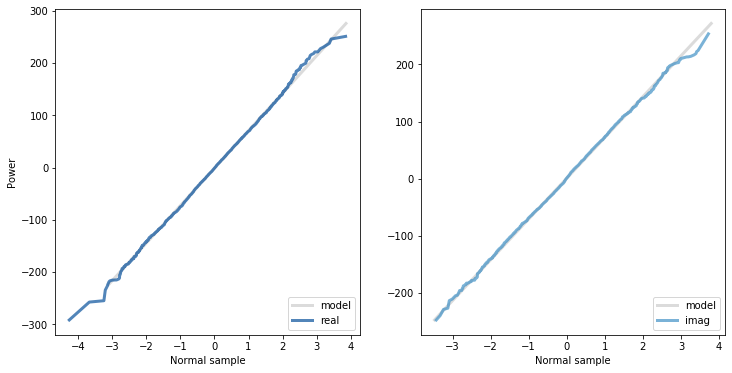
\includegraphics[width=0.75\textwidth]{13.png}
        \caption{Сравнение спектров}
        \label{fig:lab4_fig4_4}
\end{figure}

\chapter{Упражнение 4.5}

Вот весь процесс в функции: Создает розовый шум с помощью алгоритма Восса-Маккартни.

\begin{lstlisting}[caption=Создание функции]
def voss(nrows, ncols=16):
    array = np.empty((nrows, ncols))
    array.fill(np.nan)
    array[0, :] = np.random.random(ncols)
    array[:, 0] = np.random.random(nrows)
    
    # the total number of changes is nrows
    n = nrows
    cols = np.random.geometric(0.5, n)
    cols[cols >= ncols] = 0
    rows = np.random.randint(nrows, size=n)
    array[rows, cols] = np.random.random(n)

    df = pd.DataFrame(array)
    df.fillna(method='ffill', axis=0, inplace=True)
    total = df.sum(axis=1)

    return total.values
\end{lstlisting}

Чтобы проверить это, я сгенерирую 12005 значений:

\begin{lstlisting}[caption=Генерация значений]
ys = voss(12005)
ys
\end{lstlisting}

Теперь создадим из них звук:

\begin{lstlisting}[caption=Создание звука]
wave = thinkdsp.Wave(ys)
wave.unbias()
wave.normalize()
\end{lstlisting}

Теперь посмотрим на его визуализацию.

\begin{lstlisting}[caption=Визуализация звука]
wave.plot()
\end{lstlisting}

\begin{figure}[H]
        \centering
        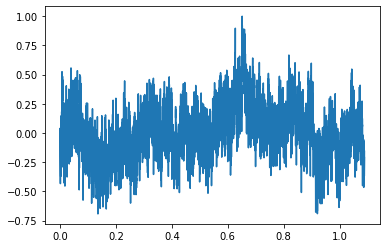
\includegraphics[width=0.75\textwidth]{14.png}
        \caption{Визуализация звука}
        \label{fig:lab4_fig5_1}
\end{figure}

Как и ожидалось, это больше похоже на случайное блуждание, чем на белый шум, но более случайное, чем на красный шум. Теперь рассмотрим спектр мощности:

\begin{lstlisting}[caption=Спектр мощности звука]
spectrum = wave.make_spectrum()
spectrum.hs[0] = 0
spectrum.plot_power()
decorate(xlabel='Frequency (Hz)',
                 xscale='log', 
                 yscale='log')
\end{lstlisting}

\begin{figure}[H]
        \centering
        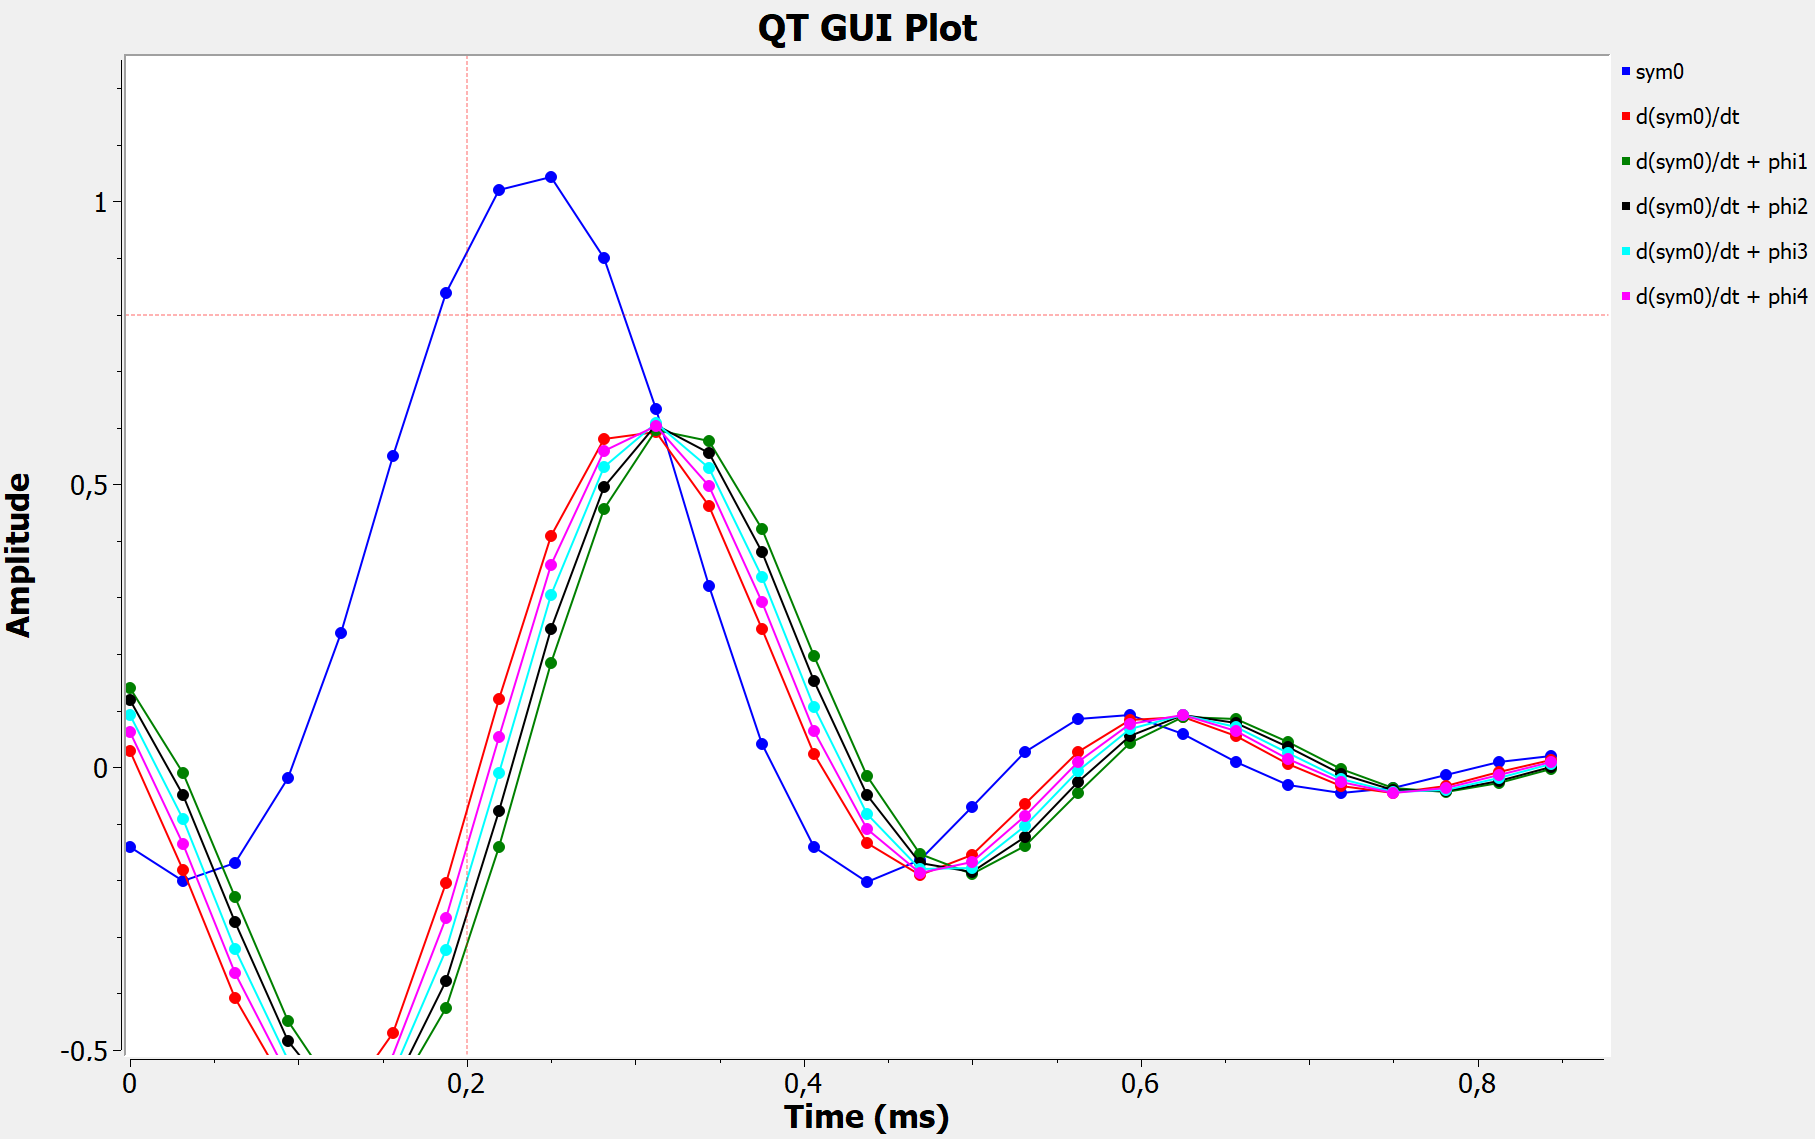
\includegraphics[width=0.75\textwidth]{15.png}
        \caption{Спектр мощности звука}
        \label{fig:lab4_fig5_2}
\end{figure}

Посмотрим на наклон:

\begin{lstlisting}[caption=Наклон прямой]
spectrum.estimate_slope().slope
\end{lstlisting}

Расчетный наклон близок к -1 (\texttt{-1.0129573459835064}).

Мы можем лучше понять средний спектр мощности, сгенерировав более длинную выборку:

\begin{lstlisting}[caption=Генерация более длинной выборки]
seg_length = 40 * 124
iters = 100
wave = thinkdsp.Wave(voss(seg_length * iters))
len(wave)
\end{lstlisting}

И используя метод Барлетта для вычисления среднего.

\begin{lstlisting}[caption=Использование метода Барлетта]
spectrum = bartlett_method(wave, length=seg_length, flag=False)
spectrum.hs[0] = 0
len(spectrum)
\end{lstlisting}

Это довольно близко к прямой линии с некоторой кривизной на самых высоких частотах, если рассматривать спектр мощности звука.

\begin{lstlisting}[caption=Спектр мощности звука]
spectrum.plot_power()
decorate(xlabel='Frequency (Hz)',
                 xscale='log', 
                 yscale='log')
\end{lstlisting}

\begin{figure}[H]
        \centering
        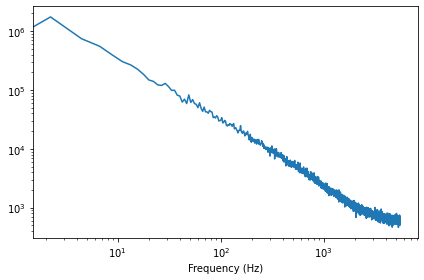
\includegraphics[width=0.75\textwidth]{16.png}
        \caption{Спектр мощности звука}
        \label{fig:lab4_fig5_3}
\end{figure}

Посмотрим на наклон:

\begin{lstlisting}[caption=Наклон прямой]
spectrum.estimate_slope().slope
\end{lstlisting}

Наклон теперь более близок к -1 (\texttt{-1.0048368551745679}).

\chapter{Выводы}

Во время выполнения лабораторной работы получены навыки работы с различными видами шумов. Также получены навыки создания этих шумов через различные данные.

\end{document}
